\documentclass[10pt,letterpaper]{article}
\usepackage[utf8]{inputenc}
\title{EV 2.2 Explicar los arreglos y parametros de los amplificadores clase A}
\author{Ascencio De Leon Agustin}
\usepackage[spanish]{babel}
\usepackage{graphicx}
\graphicspath{{ampli/}}
\usepackage[left=2.5cm,top=2.5cm,bottom=3cm,right=2.5cm]{geometry}

\begin{document}
\maketitle
\begin{figure}[h!]
\centering
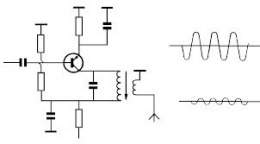
\includegraphics[scale=.9]{260px-AmplificadorclaseA}
\end{figure}
\newpage
\section{Que es un amplificador clase A}
Amplificador clase A. Son aquellos amplificador cuyas etapas de potencia consumen corrientes altas y continuas de su fuente de alimentación, independientemente de si existe señal de audio o no.

\begin{figure}[h!]
\centering
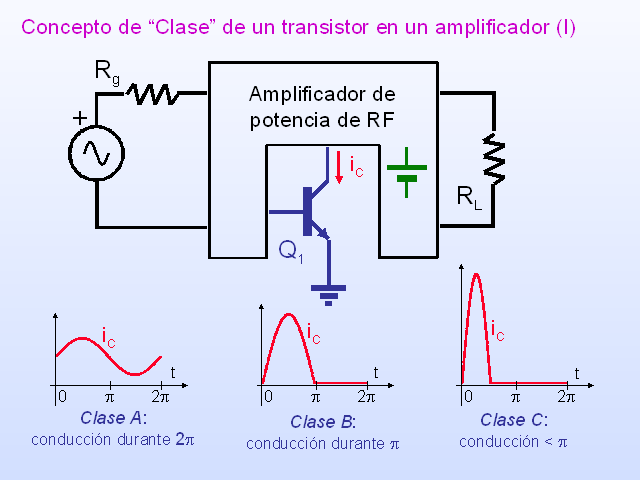
\includegraphics[scale=.5]{img2}
\end{figure}
\newpage
\section{Parámetros de dispersión}
En sistemas de RF la forma de evaluar la salida y entrada de un cuadripo10 es mediante los
términos que relacionan las ondas incidentes y reflejadas (coeficiente de reflexión, ROE,
etc.). Esto sucede, ya que en la práctica es la forma que uno tiene para medir el sistema. Es
por eso que surgieron los parámetros de dispersión para poder vincular estas características
\begin{figure}[h!]
\centering
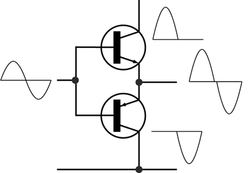
\includegraphics[scale=1]{250px-Electronic_Amplifier_Push-pull}
\end{figure}
\section{Arreglos de los amplificadores clase A}
\subsection*{El amplificador inversor}
La figura 2 ilustra la primera configuración básica del AO. El amplificador inversor. En este circuito, la entrada (+) está a masa, y la señal se aplica a la entrada (-) a través de R1, con realimentación desde la salida a través de R2.
\begin{figure}[h!]
\centering
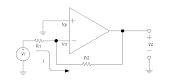
\includegraphics[scale=1.5]{unnamed}
\end{figure}
Aplicando las propiedades anteriormente establecidas del AO ideal, las características distintivas de este circuito se pueden analizar como sigue.

Puesto que el amplificador tiene ganancia infinita, desarrollará su tensión de salida, V0, con tensión de entrada nula. Ya que, la entrada diferencial de A es:

Vd = Vp - Vn, ==> Vd = 0.- Y si Vd = 0,

entonces toda la tensión de entrada Vi, deberá aparecer en R1, obteniendo una corriente en R1
 \newpage
\subsection*{El amplificador no inversor}
\begin{figure}[h!]
\centering
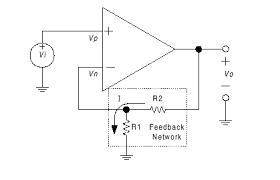
\includegraphics[scale=1]{descarga}
\end{figure}
En este circuito, la tensión Vi se aplica a la entrada (+), y una fracción de la señal de salida, Vo, se aplica a la entrada (-) a través del divisor de tensión R1 - R2. Puesto que, no fluye corriente de entrada en ningún terminal de entrada, y ya que Vd = 0, la tensión en R1 será igual a Vi. 

Así pues

 \begin{figure}[h!]
\centering
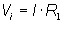
\includegraphics[scale=.9]{formula1}
\end{figure}

y como

\begin{figure}[h!]
\centering
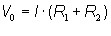
\includegraphics[scale=1]{formula2}
\end{figure}

tendremos pues que:

\begin{figure}[h!]
\centering
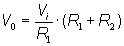
\includegraphics[scale=1]{formula3}
\end{figure}

que si lo expresamos en términos de ganancia:

\begin{figure}[h!]
\centering
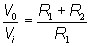
\includegraphics[scale=1]{formula4}
\end{figure}

que es la ecuación característica de ganancia para el amplificador no inversor ideal.

También se pueden deducir propiedades adicionales para esta configuración. El límite inferior de ganancia se produce cuando R2 = 0, lo que da lugar a una ganancia unidad.

En el amplificador inversor, la corriente a través de R1 siempre determina la corriente a través de R2, independientemente del valor de R2, esto también es cierto en el amplificador no inversor. Luego R2 puede utilizarse como un control de ganancia lineal, capaz de incrementar la ganancia desde el mínimo unidad hasta un máximo de infinito. La impedancia de entrada es infinita, puesto que se trata de un amplificador ideal.

\bibliography{EV_2_2_Explicar los arreglos y parametros de los amplificadores clase A}
$1.........................http://www.ifent.org/temas/amplificadores_operacionales.asp$
\linebreak
$2..........................................https://www.ecured.cu/Amplificador_clase_A$
\linebreak
$3..https://catedra.ing.unlp.edu.ar/electrotecnia/sistcom/Amplificadores/Capitulo5.pdf$

\end{document}

